\begin{titlepage}
 
\begin{tabular*}{\textwidth}%
    [b] {@{\extracolsep{0.5cm}}lr}

\begin{minipage}{0.6\textwidth}
\begin{flushleft}
% Upper part of the page
\vspace{3cm}

\includegraphics{./eeng.png}\\
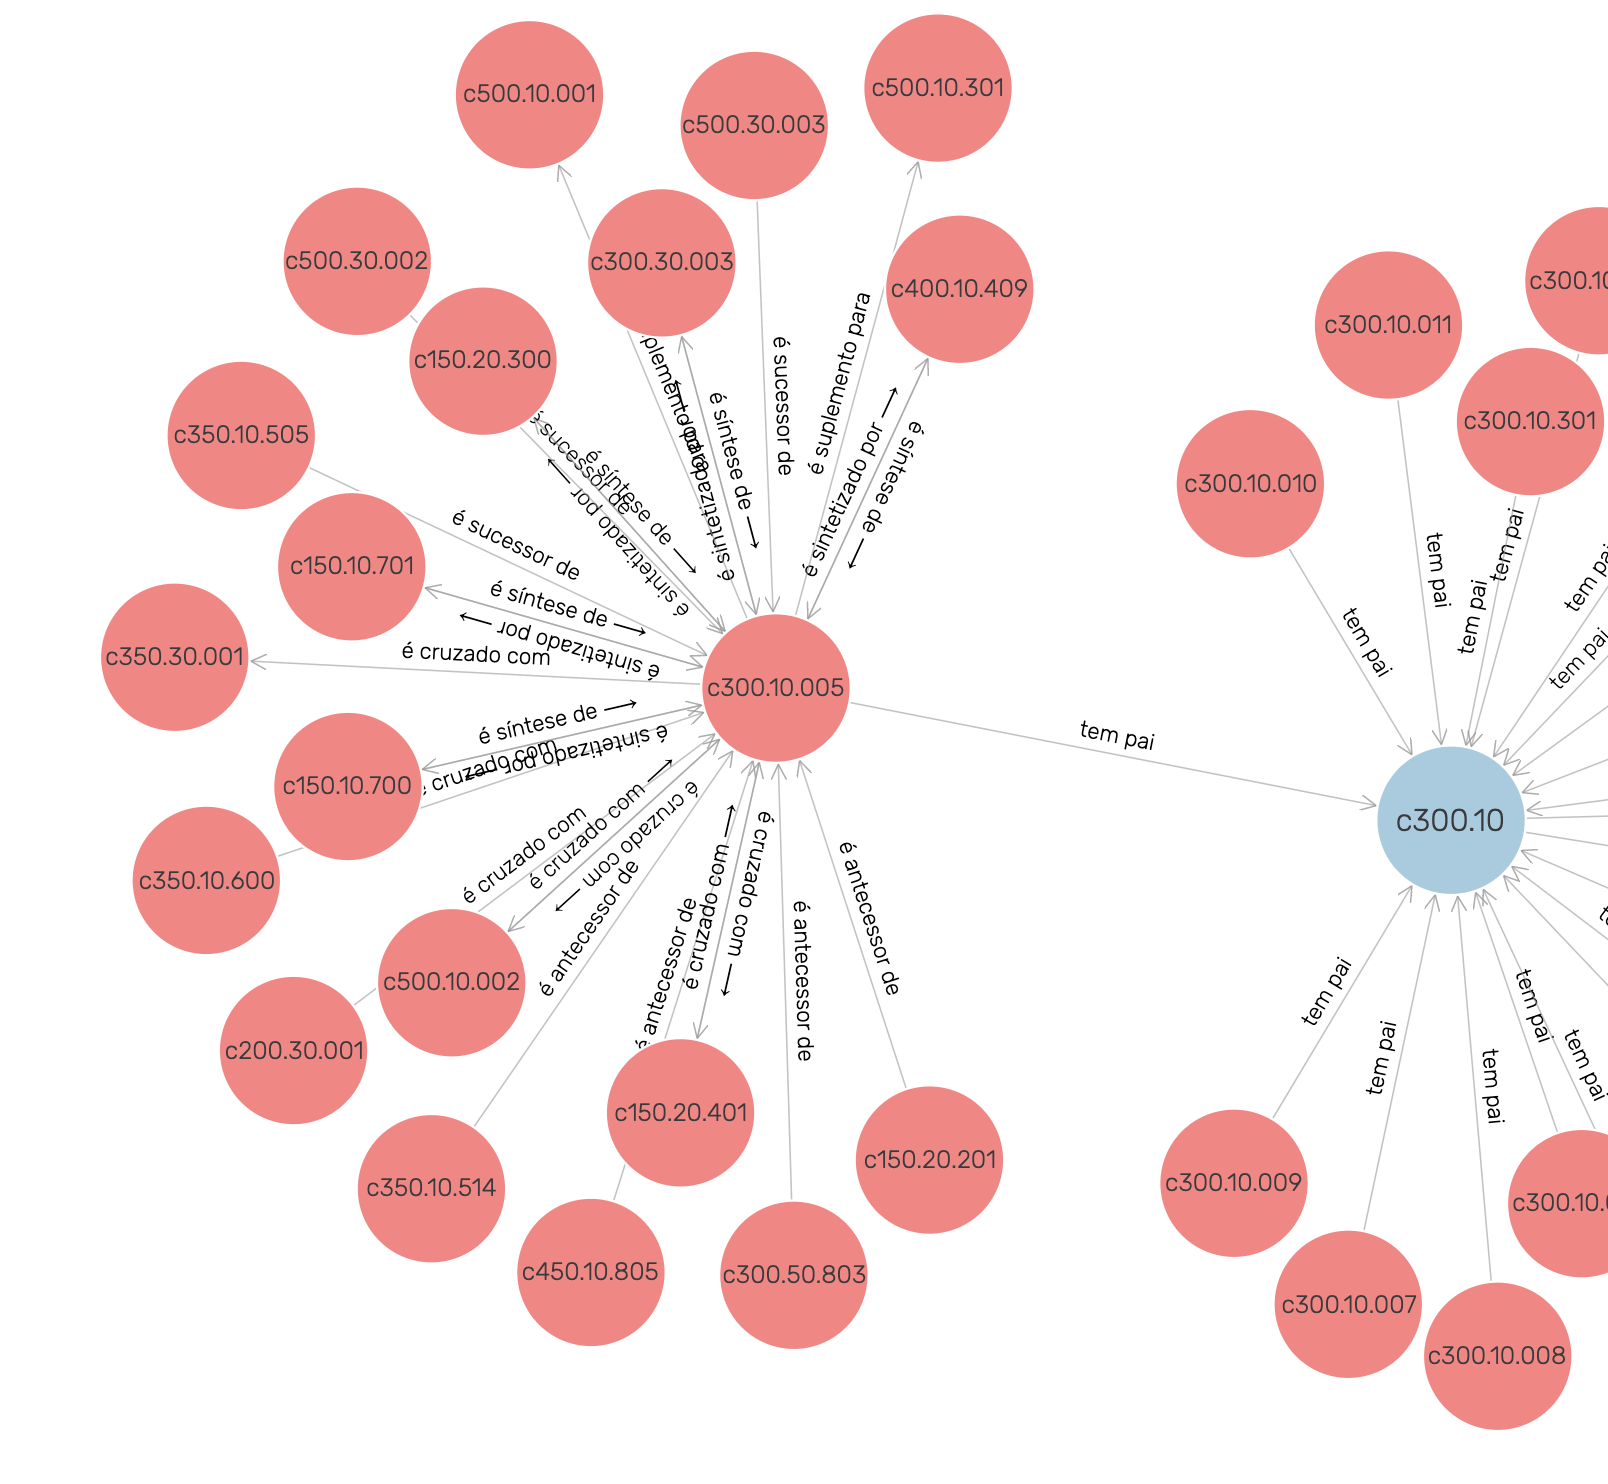
\includegraphics[width=5cm]{./onto.png}\\
\end{flushleft}
\end{minipage}

&

\begin{minipage}{0.4\textwidth}

\vspace{2cm}

 \begin{flushleft}
 
\textsc{\LARGE 
\textbf{Relatório Técnico}
}\\[1.5cm]
 
\large Requisitos de uma plataforma que auxilie na produção de atos normativos
\vspace{3cm}
\end{flushleft}
\end{minipage}

\\
\end{tabular*}

\normalsize
\begin{center}
    \begin{tabular}{l|r}
        ID Documento      & RT-\dataansi-\destsigla \\\hline
        Versão                   & 1.0 \\\hline
        Acesso                  & Restrito \\\hline
        Data de emissão & \data \\\hline
        Autor                      & José Carlos Ramalho \\\hline
        Colaborador & Luís Filipe Cunha \\\hline
        Destinatário         & \destinatario\\\hline                         
    \end{tabular}
\end{center}

 
\end{titlepage}
